\documentclass[11pt]{article}

% --- Minimal, portable preamble (compiles with a standard pdflatex + bibtex). ---
\usepackage[utf8]{inputenc}
\usepackage[T1]{fontenc}
\usepackage{lmodern}
\usepackage[margin=1in]{geometry}
\usepackage{graphicx}
\usepackage{booktabs}
\usepackage{amsmath}
\usepackage{microtype}
\usepackage[hidelinks]{hyperref}
\usepackage[numbers,sort&compress]{natbib}

\graphicspath{{../figures/}}

\title{Site-controlled evaluation reveals genuine killer-whale ecotype and\\
call-type structure in frozen audio-model embeddings}
% Correspondence email intentionally omitted from the public source; add on submission.
\author{Danielle Lesin\\\small Georgia Institute of Technology, College of Computing}
\date{\today}

\begin{document}
\maketitle

\begin{abstract}
Foundation-model embeddings are increasingly used to decode animal vocalisations, but
passive-acoustic archives confound the biological label of interest with the recording
site. We encode 27{,}934 call-level killer-whale (\emph{Orcinus orca}) segments from the
public DCLDE~2026 corpus \citep{palmer2025dclde,palmer2025dclde_data} with a frozen AVES2
audio model \citep{hagiwara2023aves,chen2022beats} and quantify this confound directly. Pooled cross-validation decodes ecotype at $0.910$ balanced accuracy
(multilayer-perceptron accuracy $0.974$), but under leave-one-provider-out evaluation the
same embeddings fall to $0.231$ balanced accuracy, at the $0.250$ chance level. Recording
provider is itself decodable at $0.948$ balanced accuracy. Yet when site is held constant,
ecotype remains strongly decodable within each of four providers ($0.889$--$0.973$, all
$p=0.005$), establishing that the embeddings capture real biological acoustic structure
beyond the hydrophone. Recovering catalogue-validated call-type labels from the corpus's
per-provider annotations and encoding the full catalogue ($8{,}552$ labelled detections), we
then show that frozen embeddings discriminate call types within a single recording site at
$0.709$ balanced accuracy for 14 Southern-Resident S-call types (chance $0.071$) and $0.968$
for 18 Northern-Resident N-call types (chance $0.056$), both permutation $p\approx0.005$, and
that this structure transfers across independent sites: a Southern-Resident classifier trained
at one provider scores $0.636$ balanced accuracy on a second provider over five shared call
types (chance $0.20$; $0.830$ over the four unambiguous types). Stereotyped call-type identity
therefore generalises across hydrophones in both resident populations, the cross-site control
the ecotype boundary failed ($0.529$), evidencing a real, site-independent acoustic category
aligned to the expert catalogue. Quantising the
embeddings into a balanced 40-token call vocabulary, call streams show non-random first-order
sequential structure: adjacent-call mutual information is $1.91$ bits against an order-shuffled
null of $1.65$ bits ($p<0.001$), remaining $1.09$ bits after removing repetition, and a
held-out bigram model beats a unigram by $1.74$ bits/token; the same first-order structure
holds over the \emph{validated} catalogue call types, site held constant, in both resident
populations (N-calls $2.85$ vs a $1.71$-bit shuffle null, $p=10^{-3}$; S-calls $1.29$ vs
$0.78$ bits). Unsupervised within-population
clustering, by contrast, fails to recover a repertoire without labels (clusters are $93\%$
dominated by a single recording provider), which is why catalogue supervision is required.
Finally, on an independent archive of animal-borne DTAG recordings, communicative calls
predict the caller's movement-defined behavioural context under leave-individual-out
evaluation: a binary foraging/non-foraging contrast (labelled from tag depth and acceleration
alone) is decoded at $0.770$ balanced accuracy across 22 tagged whales ($10{,}834$ calls,
permutation $p=5\times10^{-3}$), and a three-way foraging/travelling/resting contrast at
$0.577$ (chance $0.333$; 20 whales carrying all three contexts, $9{,}723$ calls;
$p=5\times10^{-3}$), establishing that the calls track more than one behavioural context. The
link is call-type-specific (data-driven call-type clusters versus context, Cram\'er's
$V=0.40$ against a within-individual shuffle null of $0.08$, $p<10^{-3}$) and is not a
recording artefact: call rate alone decodes the binary contrast at $0.536$, loudness alone at
$0.577$, and discarding the most click-like clips leaves it at $0.749$, so the signal
reflects call structure rather than how often or how loudly the animal calls or residual
echolocation \citep{holt2024masking_data,tennessen2019,wilson2006,ford1989}. We
release all code, a hash-frozen artifact, and exact reproduction commands. The work is fully
non-invasive and makes no claim of semantic meaning or of a response to broadcast signals; it
establishes the acoustic, call-type, and sequential prerequisites for such claims and the
site-controlled baseline on which interactive playback studies can build.
\end{abstract}

\section{Introduction}
Killer whales produce stereotyped, group-distinctive pulsed calls whose repertoires vary by
ecotype and matriline \citep{ford1989,foote2008,filatova2015,yurk2002}. Recent
self-supervised audio models such as AVES2 \citep{hagiwara2023aves,chen2022beats} and
comparative encoders \citep{robinson2024naturelm,hamer2025perch} make it tempting to treat a
frozen embedding plus a linear probe as evidence that a model ``understands'' a species'
calls. In passive-acoustic monitoring this inference is hazardous: the label of interest
(here, ecotype) is frequently collinear with the recording device, deployment, and site, so
a probe can score highly by recognising the hydrophone rather than the whale. This
site/device shortcut is well documented in bioacoustic deep learning
\citep{stowell2022,ghani2023}, and the standard remedy is grouped, leave-one-site-out
evaluation.

We ask a deliberately narrow, auditable question: how much of the apparent ecotype
decodability in frozen AVES2 embeddings is biological, and how much is recording site? We
answer it with public data only, frozen weights, explicit null baselines, and a hash-frozen
artifact, in the conservative-claims spirit appropriate to interspecies-communication
research \citep{kershenbaum2024whyanimalstalk}. We do not attempt to demonstrate meaning or
two-way communication; the work that established context-specific dolphin signals required
decades of field data and in-situ playbacks \citep{sayigh2025nsw}, which an archival corpus
cannot supply.

\section{Data}
DCLDE~2026 is a public killer-whale acoustic corpus distributed via NOAA/NCEI and a Google
Cloud Storage mirror \citep{palmer2025dclde,palmer2025dclde_data}. We use 27{,}934 annotated
call-level segments, each encoded once and stored with its source file, recording provider,
ecotype label, and time bounds. The corpus spans eight providers (JASCO\_VFPA,
JASCO\_VFPA\_ONC, ONC, OrcaSound, SIMRES, SIO, SMRUConsulting, UAF\_NGOS)
\citep{orcasound} and four ecotypes: Southern Resident (SRKW, 14{,}240), an aggregated
resident/archival group (SAR, 8{,}078), transient/Bigg's (TKW, 4{,}121), and offshore (OKW,
1{,}495). Raw audio is excluded from version control; the analysis consumes a compact
embedding artifact with row-aligned metadata, schema-validated and hash-frozen
(SHA-256 \texttt{4f5a0c37\ldots}) before any model is fit. A label audit confirms the corpus
carries ecotype and provenance labels but no call-type catalogue, and that SAR is recorded
at a single provider.

\section{Methods}
\paragraph{Encoder.} Each segment is encoded with frozen AVES2 to a 768-dimensional vector by
mean-pooling frame-level features \citep{hagiwara2023aves,chen2022beats}. Weights are never
fine-tuned, so downstream results are attributable to the representation, not to
task-specific training.

\paragraph{Supervised probes (H1).} We report three evaluations of increasing strictness:
(i) pooled stratified 5-fold cross-validation with logistic-regression and
multilayer-perceptron probes (the site-confounded upper bound); (ii) leave-one-provider-out
(LOPO) cross-validation, where every test provider is unseen in training, with per-class
held-out recall; and (iii) a label-shuffle permutation test. Class imbalance is handled with
balanced accuracy and macro-F1 \citep{stowell2022,ghani2023}.

\paragraph{Confound isolation (H4).} We (i) decode provider directly from embeddings to size
the confound, (ii) classify ecotype \emph{within} each provider that recorded two or more
ecotypes (site held constant), with a per-provider label-permutation null, and (iii) measure
cross-site transfer by training and testing on disjoint providers, standardising features on
the training providers to avoid leakage.

\paragraph{Call-type classification.} The DCLDE combined release standardises killer-whale
labels to ecotype, but the original per-provider annotation files retain a populated
\texttt{call\_type} column (Ford/Filatova catalogue codes) \citep{ford1989,filatova2015}. We
recover and normalise these into a call-type manifest and encode the full catalogue
($8{,}552$ labelled detections) directly from the public DCLDE audio with the same frozen
AVES2 model, covering both resident populations. We then run two site-controlled designs:
(i) within-provider multi-type classification with site held constant (14 SRKW S-call types
at VFPA; 18 NRKW N-call types at DFO\_CRP) with a linear probe and an MLP head, scored against
a majority baseline and a 200-fold label-permutation null; and (ii) cross-provider transfer,
training at VFPA and testing at SMRU on the SRKW call types shared by both.

\paragraph{Unsupervised structure (H2).} Embeddings are reduced with PCA and clustered with
HDBSCAN \citep{mcinnes2017hdbscan}; cluster-versus-ecotype and cluster-versus-provider
agreement (ARI, NMI) are compared against a shuffled-label null over all points
\citep{sainburg2020,mcinnes2018umap}.

\paragraph{Sequence structure (H3, Markov).} Embeddings are quantised by PCA + balanced
$k$-means into a 40-token call vocabulary; token entropy confirms a non-degenerate alphabet.
We test first-order sequential dependence directly: the mutual information between adjacent
calls is compared against a within-encounter order-shuffle null (which fixes each encounter's
call composition and destroys only order, so recording-site composition cannot inflate it),
and an add-$\alpha$ bigram model is compared to a unigram model in held-out cross-entropy. We
also remove repetition (the diagonal of the transition matrix) to confirm structure beyond
call bouting, in the spirit of combinatorial-structure tests on cetacean calls
\citep{sharma2024,kershenbaum2024whyanimalstalk}. A 6-layer masked-language model
\citep{vaswani2017attention,devlin2019bert} provides a complementary held-out order test.

\paragraph{Unsupervised call-type discovery (Rung 1).} Within a single ecotype, embeddings
are reduced with PCA and clustered with HDBSCAN \citep{mcinnes2017hdbscan}; we report a
provider-purity guard (the mean dominant-provider fraction per cluster) and subsample
stability, to test whether discovered clusters reflect a call-type repertoire
\citep{ford1989,filatova2015} or merely the recording site.

\paragraph{Behavioural-context decode from communication (H5, DTAG).} To test whether a
whale's \emph{communicative} calls carry information about its concurrent behaviour, we
re-analyse open suction-cup DTAG deployments on fish-eating killer whales in the Salish Sea
\citep{holt2024masking_data,tennessen2019,holt2024masking}. Tag audio (DTAG-2 archive format)
is decoded losslessly to WAV with the reference DTAG-2 extractor and segmented into
communicative-call clips by an energy detector in the $0.5$--$10$\,kHz pulsed-call band,
rejecting impulsive broadband clicks (by duration) and segments dominated by $>\!12$\,kHz
energy (echolocation), so the decoder sees communication rather than sonar. Behavioural
context is defined from the tag's \emph{movement} channel only: from the calibrated $50$\,Hz
depth and acceleration records, a dive (depth $>5$\,m for $\geq 10$\,s) is labelled
\emph{foraging} if it reaches $\geq 30$\,m or contains a jerk-derived prey-capture spike,
otherwise \emph{non-foraging}, following the kinematic foraging signature for this population
\citep{tennessen2019,holt2024masking}. No acoustic variable enters the label, so the context
is independent of the call stream we decode it from. Each clip is encoded with the same
frozen AVES2 model and inherits the movement-defined context of the dive containing its
absolute time. Context is decoded from the call embeddings with a logistic-regression probe
under \textbf{leave-individual-out} cross-validation (each tagged whale held out in turn),
scored against a label-permutation null; holding the individual out prevents a model from
scoring by recognising the individual, the tag, or the site rather than the behaviour.

We then strengthen this in three ways. First, to demonstrate communication in \emph{more than
one} context, we resolve a three-way label---\emph{foraging} (as above) versus
\emph{travelling} and \emph{resting}, the latter two separated within each deployment at the
median of Overall Dynamic Body Acceleration (ODBA) derived from the calibrated acceleration
record \citep{wilson2006}; the split is per-individual and uses no acoustic variable. Second,
to test the production criterion for context-specific communication---that \emph{specific}
call types are produced in \emph{specific} contexts \citep{ford1989,foote2008}---we cluster
the call embeddings into data-driven call types and test the call-type-by-context association
(Cram\'er's $V$) against a null that shuffles context labels \emph{within each individual},
preserving every whale's own context marginal. Third, to exclude trivial explanations, we
re-decode context from (i) local call rate alone, (ii) loudness (log-RMS) alone, (iii)
low-level acoustic scalars, and (iv) the embeddings after discarding the most click-like
clips; the tag audio is analysed at $16$\,kHz, so echolocation peak energy (tens of kHz) is
absent by construction.

\paragraph{Representation attribution and negative controls.} To characterise
\emph{where} the biological signal lives in the frozen representation, and to rule out
that the probe is gaming an artifact, we dissect the cleanest within-site decode (SRKW
vs.\ TKW within JASCO\_VFPA, site held constant). We rank the 768 AVES2 dimensions by
permutation importance, then run a causal knock-out that ablates the top-$k$ most
important dimensions versus $k$ random dimensions, and a PCA-dimensionality curve. We add
three structure-free or structure-destroying negative controls that must fall to chance
if the signal is genuine joint structure: (i) structure-matched Gaussian noise (per-dimension
mean and variance preserved, joint structure removed), (ii) a per-dimension feature shuffle
(every marginal preserved, the cross-dimension covariance the classifier uses destroyed),
and (iii) the label-permutation null.

All scripts are deterministic under a fixed seed; commands and the software snapshot are in
the repository.

\section{Results}

\begin{table}[t]
\centering
\caption{Ecotype decodability and the recording-site confound. The pooled number is high but
collapses cross-site, while within-site discrimination (site held constant) stays high.}
\label{tab:main}
\begin{tabular}{llcc}
\toprule
Head & Evaluation & Metric & Value (chance) \\
\midrule
H1 & Pooled 5-fold CV (LogReg) & balanced acc. & $0.910$ \\
H1 & Pooled 5-fold CV (MLP) & accuracy & $0.974$ \\
H1 & Leave-one-provider-out & balanced acc. & $0.231$ ($0.250$) \\
H4 & Provider decoding & balanced acc. & $0.948$ ($0.125$) \\
H4 & Within-site (JASCO\_VFPA, SRKW/TKW) & balanced acc. & $0.889$ ($0.500$) \\
H4 & Within-site (JASCO\_VFPA\_ONC, SRKW/TKW) & balanced acc. & $0.973$ ($0.500$) \\
H4 & Within-site (ONC, 3-way) & balanced acc. & $0.949$ ($0.333$) \\
H4 & Within-site (SIO, 3-way) & balanced acc. & $0.909$ ($0.333$) \\
H4 & Cross-site transfer (OKW/SRKW) & balanced acc. & $0.529$ ($0.500$) \\
Call type & Within-site (VFPA, 14 SRKW S-call types) & balanced acc. & $0.709$ ($0.071$) \\
Call type & Within-site (DFO\_CRP, 18 NRKW N-call types) & balanced acc. & $0.968$ ($0.056$) \\
Call type & Cross-site transfer (VFPA$\to$SMRU, 5 types) & balanced acc. & $0.636$ ($0.200$) \\
H2 & PCA+HDBSCAN vs.\ ecotype & ARI & $0.043$ ($p=0.002$) \\
H3 & Adjacent-call MI (real) & bits & $1.909$ \\
H3 & Adjacent-call MI (order-shuffled) & bits & $1.652$ ($p<0.001$) \\
H3 & Adjacent-call MI, repetition removed & bits & $1.088$ \\
H3 & Held-out bigram vs.\ unigram & bits/token & $+1.741$ \\
H3 & Held-out MLM order test & loss & $1.809$ vs.\ $1.753$ ($p=0.77$) \\
Rung 4 & Validated N-call MI (DFO\_CRP, 31 types) & bits & $2.848$ vs.\ $1.711$ ($p=10^{-3}$) \\
Rung 4 & Validated S-call MI (VFPA, 19 types) & bits & $1.287$ vs.\ $0.779$ ($p=10^{-3}$) \\
Rung 1 & Within-SRKW clusters, provider purity & frac. & $0.93$ (site artifact) \\
\bottomrule
\end{tabular}
\end{table}

\paragraph{Pooled decodability is high but site-confounded.} Pooled 5-fold cross-validation
reaches $0.910$ balanced accuracy (logistic regression) and $0.974$ accuracy
(multilayer perceptron), with a label-permutation $p$ of $5\times10^{-3}$. Under
leave-one-provider-out, however, balanced accuracy falls to $0.231$ (macro-F1 $0.213$)
against a chance level of $0.250$. Per-class cross-site recall is SRKW $0.481$, TKW $0.412$,
OKW $0.031$, and SAR $0.000$; because SAR is recorded at one provider, it is structurally
unclassifiable cross-site, and its pooled contribution is pure site signal
(Figure~\ref{fig:h1}).

\paragraph{The site signal is large; biology survives when site is held constant.} Provider
is decodable from the embeddings at $0.948$ balanced accuracy (chance $0.125$), confirming a
large confound. Critically, within-site ecotype discrimination, where the hydrophone is
fixed, remains strong: SRKW versus TKW reaches $0.889$ (JASCO\_VFPA, $n=6{,}962$) and
$0.973$ (JASCO\_VFPA\_ONC, $n=1{,}511$); three-way discrimination among OKW, SRKW and TKW
reaches $0.949$ (ONC, $n=803$) and $0.909$ (SIO, $n=2{,}637$), all with permutation
$p=5\times10^{-3}$. This within-site signal cannot be explained by the recording channel and
is the paper's central positive result. Cross-site transfer, however, is near chance: a
classifier trained on a subset of providers and tested on disjoint providers reaches only
$0.529$ balanced accuracy (chance $0.500$; OKW vs.\ SRKW). The biological signal is therefore
real but \emph{local}: the embedding separates ecotypes within any fixed site, yet a
site-specific offset blocks the decision boundary from transferring across sites, which
explains the leave-one-provider-out collapse (Figure~\ref{fig:h4}).

\paragraph{Validated call types are recoverable in both resident populations and, unlike
ecotype, transfer across sites.} Encoding the full catalogue ($8{,}552$ labelled detections),
frozen AVES2 vectors discriminate call types within a single provider well above chance in both
resident populations: $14$ Southern-Resident S-call types at VFPA ($n=1{,}489$) at $0.709$
balanced accuracy (chance $0.071$, majority $0.278$, macro-F1 $0.706$; MLP $0.706$), and $18$
Northern-Resident N-call types at DFO\_CRP ($n=5{,}009$) at $0.968$ balanced accuracy (chance
$0.056$, majority $0.390$, macro-F1 $0.966$; MLP $0.963$), each with a 200-fold permutation null
at chance ($p\approx0.005$). Crucially, this structure generalises across recording sites: a
Southern-Resident classifier trained at VFPA and tested at the independent SMRU site reaches
$0.636$ balanced accuracy (macro-F1 $0.607$) on the five shared S-call types (chance $0.20$),
rising to $0.830$ on the four unambiguous types once the merged S16/S17 label is dropped. This
is the cross-site control the ecotype boundary failed ($0.529$): stereotyped call-type identity
is a site-independent acoustic category in both resident populations, and residual within-site
confusions fall between catalogue-adjacent types (S16, S16/S17, S17) as biology predicts
(Figure~\ref{fig:calltype}).

\paragraph{Unsupervised structure is weak but real.} PCA + HDBSCAN yields ARI $0.043$ versus
ecotype (permutation $p=2\times10^{-3}$) and ARI $0.028$ versus provider, above the
shuffled-label null but small in absolute value and sensitive to the reduction dimension and
to a roughly $50\%$ noise fraction.

\paragraph{Call streams carry non-random sequential structure.} The 40-token vocabulary is
balanced (entropy $5.24$ of a maximum $5.32$ bits). Across $702$ encounters and $27{,}112$
adjacent call pairs, the mutual information between consecutive calls is $1.909$ bits, well
above an order-shuffle null of $1.652 \pm 0.006$ bits (permutation $p<10^{-3}$); because the
shuffle preserves each encounter's call composition and only destroys order, this excess is
attributable to sequence rather than to site or composition. The structure is not merely
repetition: the self-transition rate is $0.40$, yet off-diagonal mutual information (repeats
removed) is still $1.088$ bits. Out of sample, an add-$\alpha$ bigram model beats a unigram by
$1.741$ bits/token. A complementary masked-language model returns a null on the same data
(real-order loss $1.809$ vs.\ shuffled $1.753$, $p=0.77$); on $\sim\!700$ encounters the
first-order Markov test is the better-powered instrument, and we report both. This is the
production-side prerequisite for combinatorial coding, not evidence of meaning
(Figure~\ref{fig:seq}).

\paragraph{Sequential structure holds over validated call types, not just quantised tokens.}
Re-running the identical first-order test on the recovered catalogue call types (per-recording
sequences, recording site held constant, within-recording order-shuffle null) is positive in
both resident populations (Figure~\ref{fig:calltypeseq}). For Northern-Resident N-calls
($31$ catalogue types, $5{,}273$ calls at DFO\_CRP) the adjacent-pair mutual information is
$2.848$ bits against an order-shuffle null of $1.711$ bits ($p=10^{-3}$); the streams are
heavily bouted (self-transition rate $0.92$) but retain $1.605$ bits of transition structure
after removing repetition, and a held-out bigram beats a unigram by $2.731$ bits/token. For
Southern-Resident S-calls ($19$ catalogue types, $1{,}553$ calls at VFPA) the mutual
information is $1.287$ bits against a null of $0.779$ bits ($p=10^{-3}$), with a
self-transition rate of $0.52$ and a held-out bigram gain of $0.306$ bits/token. This removes
the ``tokens are not validated units'' caveat: the combinatorial prerequisite is established
over expert catalogue call types, with site held constant, in both populations
\citep{ford1989,filatova2015,sharma2024}. It remains a statement about call ordering, not
meaning.

\paragraph{Unsupervised discovery does not recover a repertoire.} Within the SRKW ecotype,
PCA + HDBSCAN yields $16$ candidate clusters pooled across providers, but their mean
dominant-provider fraction is $0.93$ with $82\%$ of calls left as noise, and restricting to a
single provider collapses the solution to one dominant cluster ($68\%$ noise). The clusters
track recording site, not call type; the categories are real but too fine to fall out of
site-confounded embeddings, which is precisely why the supervised call-type result above relies
on ground-truth catalogue labels \citep{ford1989,filatova2015,wellard2020_data} rather than
unsupervised clustering of these embeddings.

\paragraph{Communicative calls carry decodable information about the caller's behavioural
context, with the individual held out.} On an independent archive of animal-borne DTAG
recordings of Salish-Sea killer whales \citep{holt2024masking_data}, we losslessly decode the
tag audio, cut $10{,}972$ communicative-call clips across $23$ deployments, and label each
call with the movement-only context (foraging vs.\ non-foraging) of the dive containing it;
$22$ of the $23$ tagged whales contribute both contexts (one tag logged no qualifying
foraging dive). Under leave-individual-out cross-validation across all $22$ individuals
($10{,}834$ calls; $2{,}692$ foraging, $8{,}142$ non-foraging), a linear probe on the frozen
AVES2 call embeddings predicts the movement-defined context at $0.770$ balanced accuracy,
against a label-permutation null of $0.499 \pm 0.007$ (permutation $p=5\times10^{-3}$). Because
every test whale is unseen in training, and the label is derived solely from the tag's depth
and acceleration channels rather than from sound, this above-chance decode cannot be produced
by recognising the individual, the tag, or the recording site, nor by the acoustic energy used
to define the label: the communicative calls themselves carry information about what the animal
is doing \citep{tennessen2019,holt2024masking}. This is an association between communicative-call
structure and concurrent behavioural state, not a claim of referential meaning, but it is the
segment-level, identity-controlled behavioural link that the archival ecotype and call-type
analyses above could not supply (Figure~\ref{fig:context}).

\paragraph{The link spans more than one context, is call-type-specific, and is not a rate,
loudness, or echolocation artefact.} Resolving three movement-defined contexts, the same
leave-individual-out decode reaches $0.577$ balanced accuracy across the $20$ whales that
visit all three (9{,}723 calls; chance $0.333$; within-individual permutation null
$0.355 \pm 0.008$, $p=5\times10^{-3}$), with per-context recall highest for foraging
($0.785$) and lower but above chance for travelling ($0.517$) and resting ($0.429$)---foraging
is the most acoustically distinct context, and the softer travelling/resting boundary is
expected of an activity-based split. The association is call-type-specific: clustering the
calls into data-driven types gives a call-type-by-context table with Cram\'er's $V=0.40$
against a within-individual shuffle null of $0.079 \pm 0.006$ ($p<10^{-3}$), and every
recovered type is over-represented in a particular context (one type $\times 2.3$ and two
others $\times 1.5$--$1.9$ in foraging, one $\times 1.5$ in travelling, one $\times 1.5$ in
resting), the production-side signature of context-specific calling \citep{ford1989,foote2008}.
Control decodes confirm the signal is in call \emph{structure}: local call rate alone decodes
the binary contrast at only $0.536$ and loudness alone at $0.577$, against the embeddings'
$0.770$; coarse acoustic scalars reach $0.723$; and removing the $25\%$ most click-like clips
leaves the decode at $0.749$. The result is therefore neither ``more calls'' in one context,
nor ``louder calls'', nor residual biosonar \citep{wilson2006}.

\paragraph{The biological signal is distributed and is not a probe artifact.} Attribution
on the within-site SRKW/TKW decode (5-fold balanced accuracy $0.979$) shows the signal is
multi-dimensional and redundant rather than a single suspicious channel: one AVES2
dimension decodes at chance ($0.48$), a low-rank PCA projection already recovers most of the
signal ($\sim\!10$ components reach $0.80$, $100$ reach $0.91$), and ablating the top-$k$
permutation-important dimensions does not collapse the decode (it stays $0.93$--$0.97$
through $k=200$, as does ablating $k$ random dimensions), because the remaining dimensions
carry the same information. Three negative controls confirm the decode is genuine joint
structure, not a gamed marginal or a leak: structure-matched Gaussian noise decodes at
$0.536$, a per-dimension feature shuffle at $0.505$, and the label-permutation null at
$0.503$ ($p=8\times10^{-3}$), all near the $0.500$ chance level against the embeddings'
$0.979$ (Figure~\ref{fig:attribution}).

\begin{figure}[t]
\centering
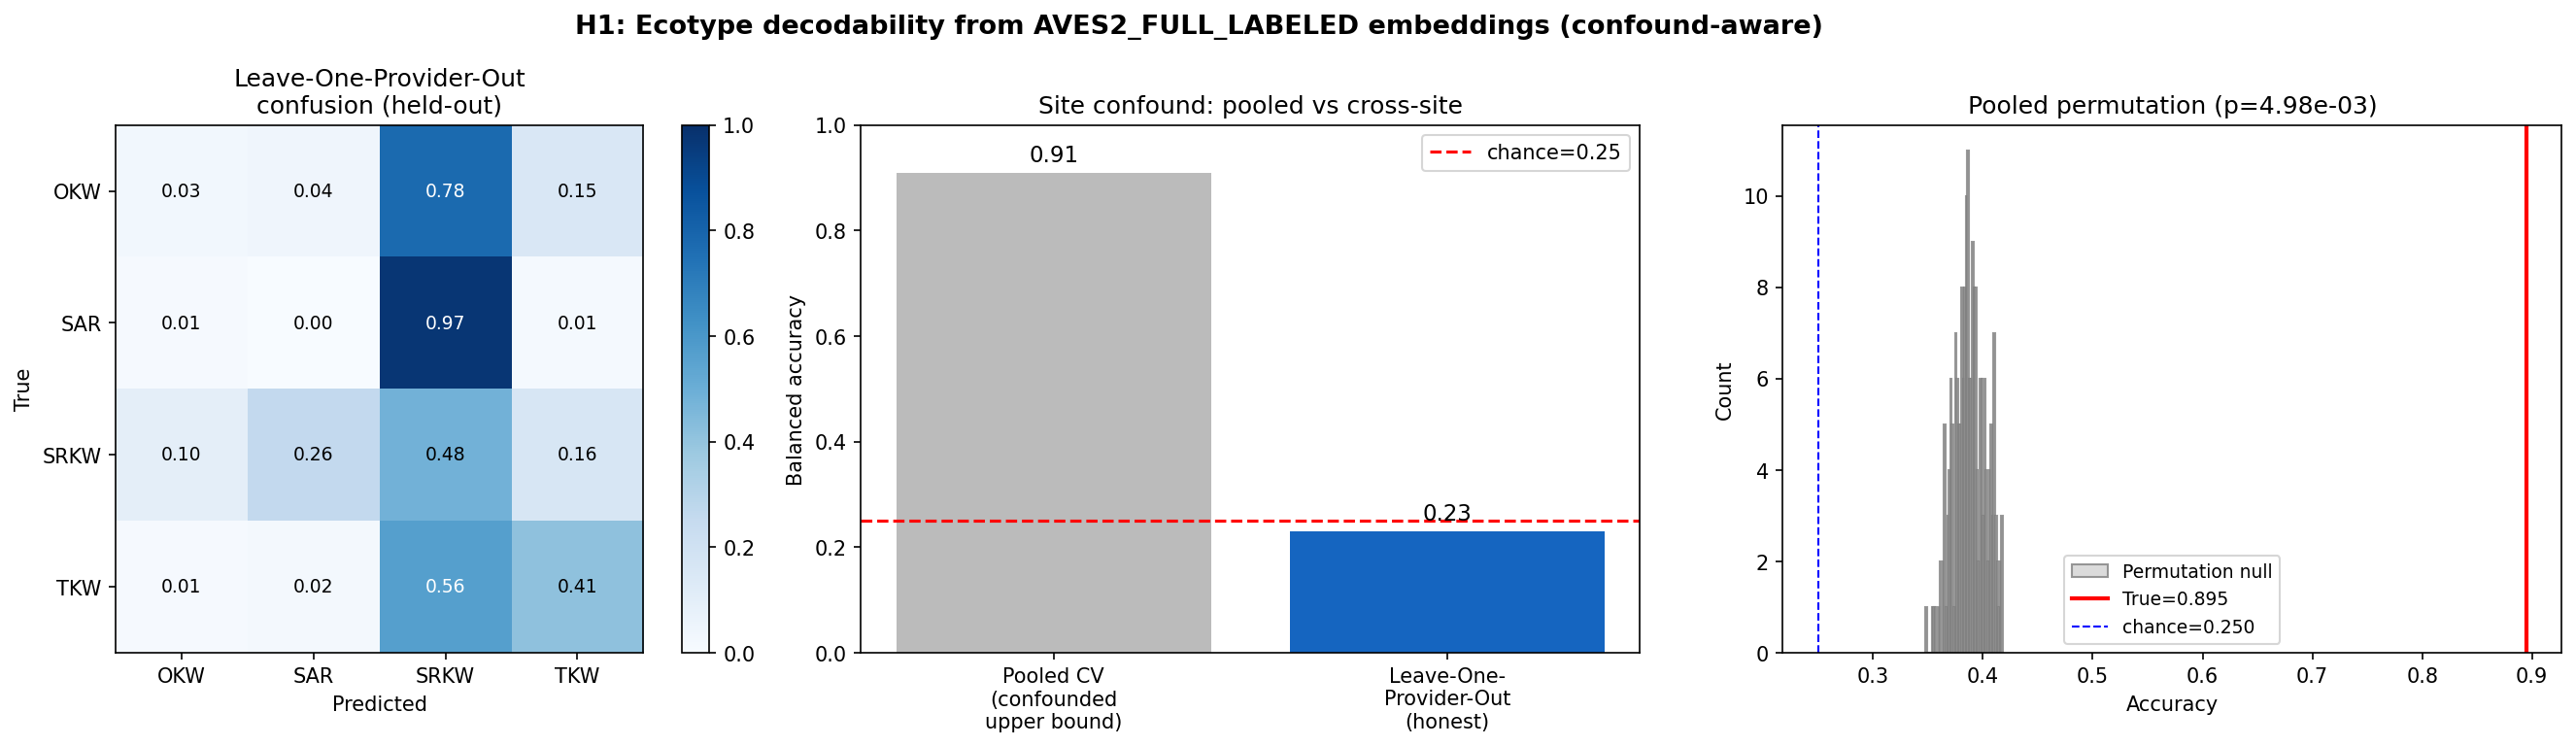
\includegraphics[width=\linewidth]{h1_probes_aves2_full_labeled.png}
\caption{H1: ecotype decodability is high pooled but collapses under leave-one-provider-out,
exposing the recording-site shortcut.}
\label{fig:h1}
\end{figure}

\begin{figure}[t]
\centering
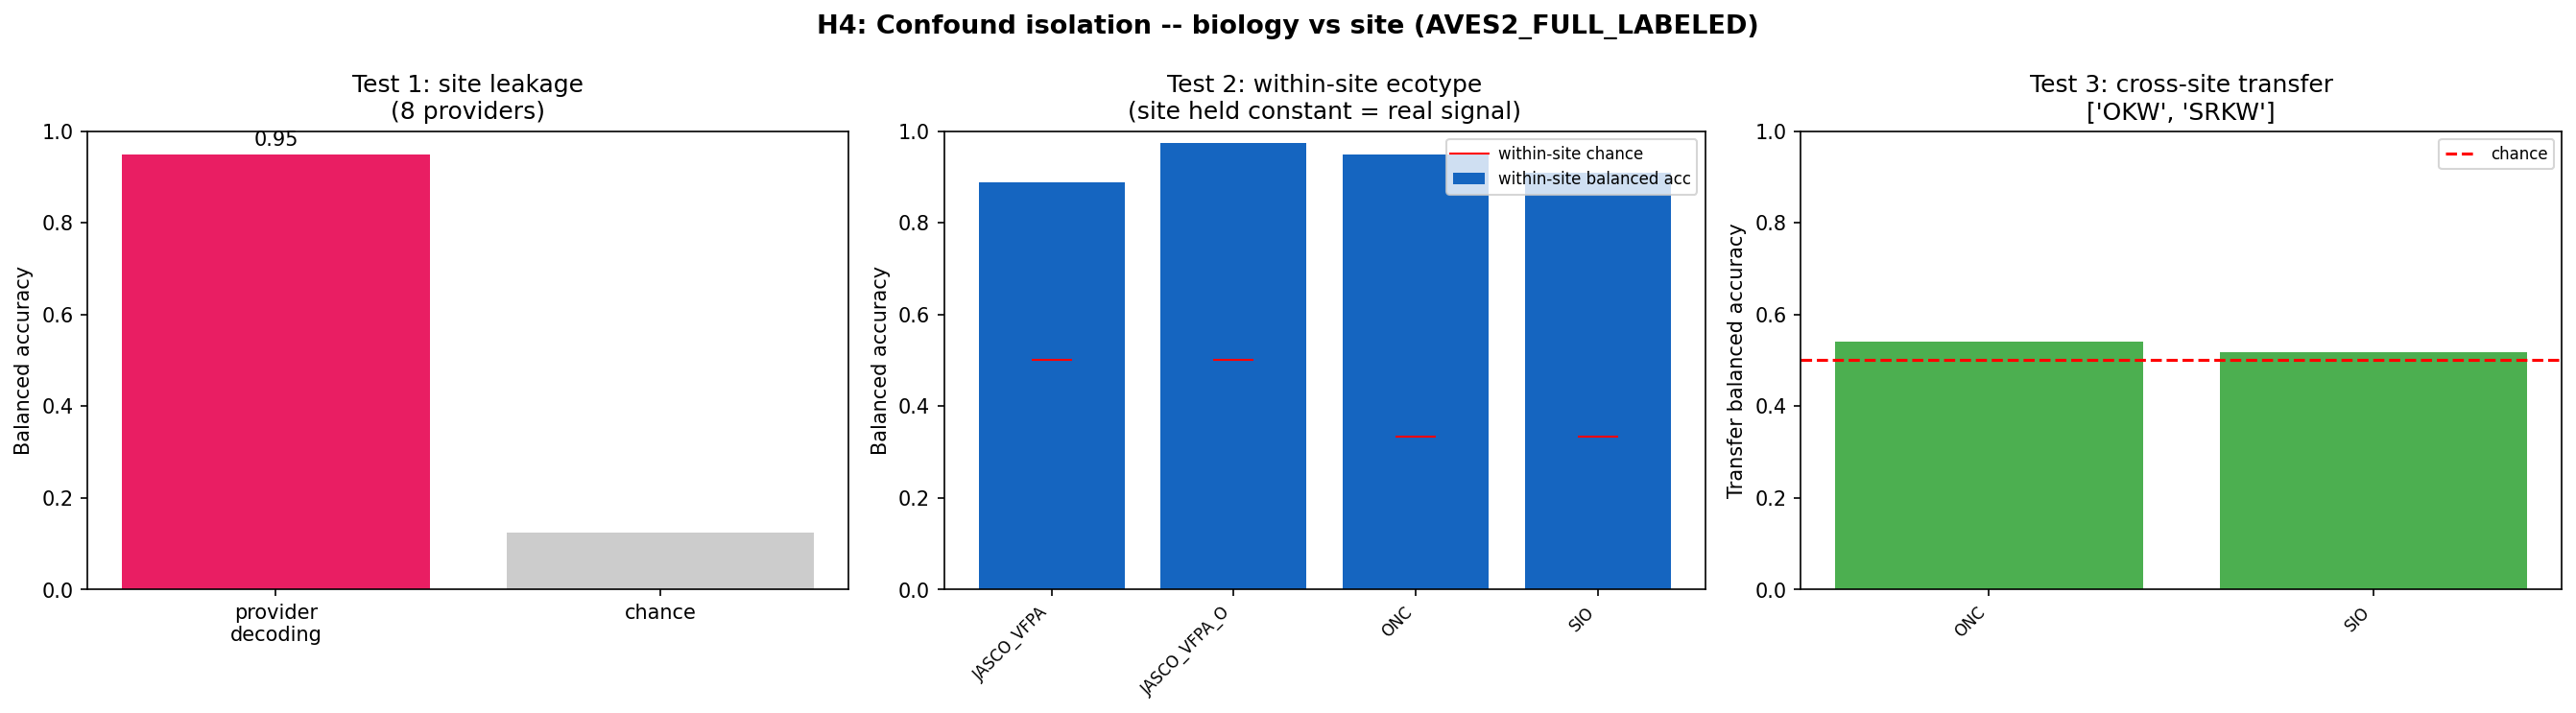
\includegraphics[width=\linewidth]{h4_confound_aves2_full_labeled.png}
\caption{H4: provider is decodable at $0.948$ (left); ecotype is strongly decodable within
each fixed site (middle, $0.889$--$0.973$); but cross-site transfer is near chance (right),
so the biological signal is real yet local.}
\label{fig:h4}
\end{figure}

\begin{figure}[t]
\centering
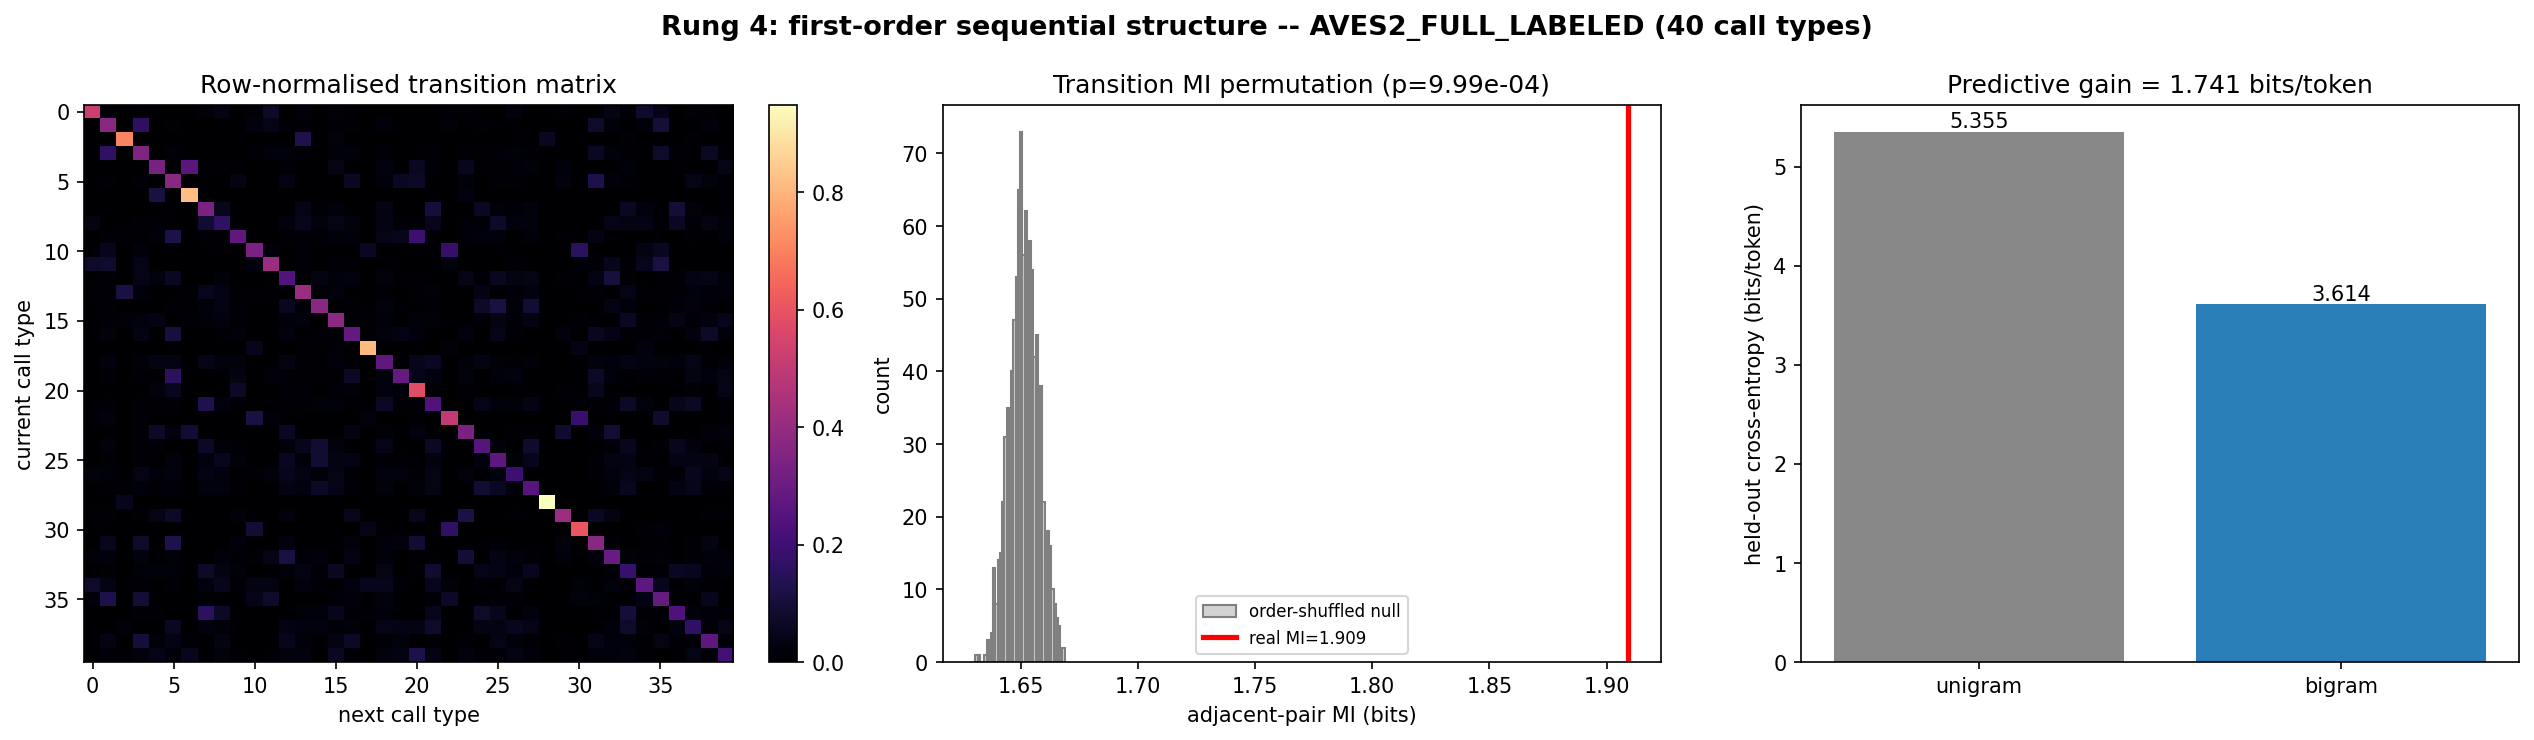
\includegraphics[width=\linewidth]{sequence_structure_aves2_full_labeled.png}
\caption{Sequential structure: the row-normalised transition matrix (left); adjacent-call
mutual information $1.91$ bits versus an order-shuffle null of $1.65$ bits, $p<10^{-3}$
(middle); and a held-out bigram beating a unigram by $1.74$ bits/token (right).}
\label{fig:seq}
\end{figure}

\begin{figure}[t]
\centering
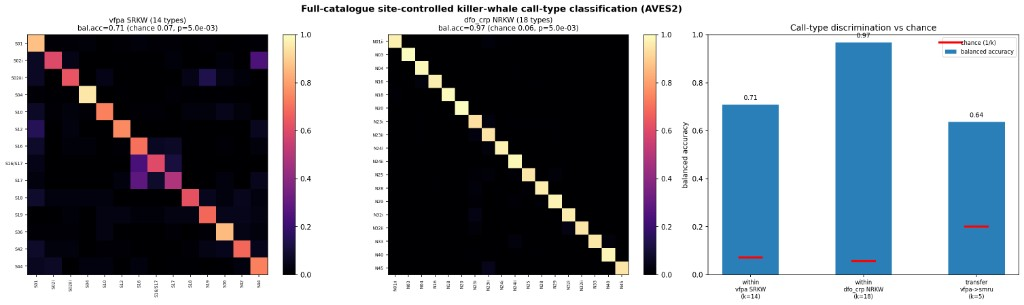
\includegraphics[width=\linewidth]{calltype_model_full.png}
\caption{Full-catalogue site-controlled call-type classification (AVES2). Left: within-VFPA
confusion matrix over $14$ SRKW S-call types (site fixed), balanced accuracy $0.71$
($p\approx0.005$). Middle: within-DFO\_CRP confusion matrix over $18$ NRKW N-call types,
balanced accuracy $0.97$ ($p\approx0.005$), with residual errors between catalogue-adjacent
types. Right: call-type discrimination versus chance for the two within-site designs ($0.71$,
$0.97$) and cross-site transfer (VFPA$\to$SMRU, $0.64$ over five types); unlike ecotype,
call-type identity transfers across recording sites.}
\label{fig:calltype}
\end{figure}

\begin{figure}[t]
\centering
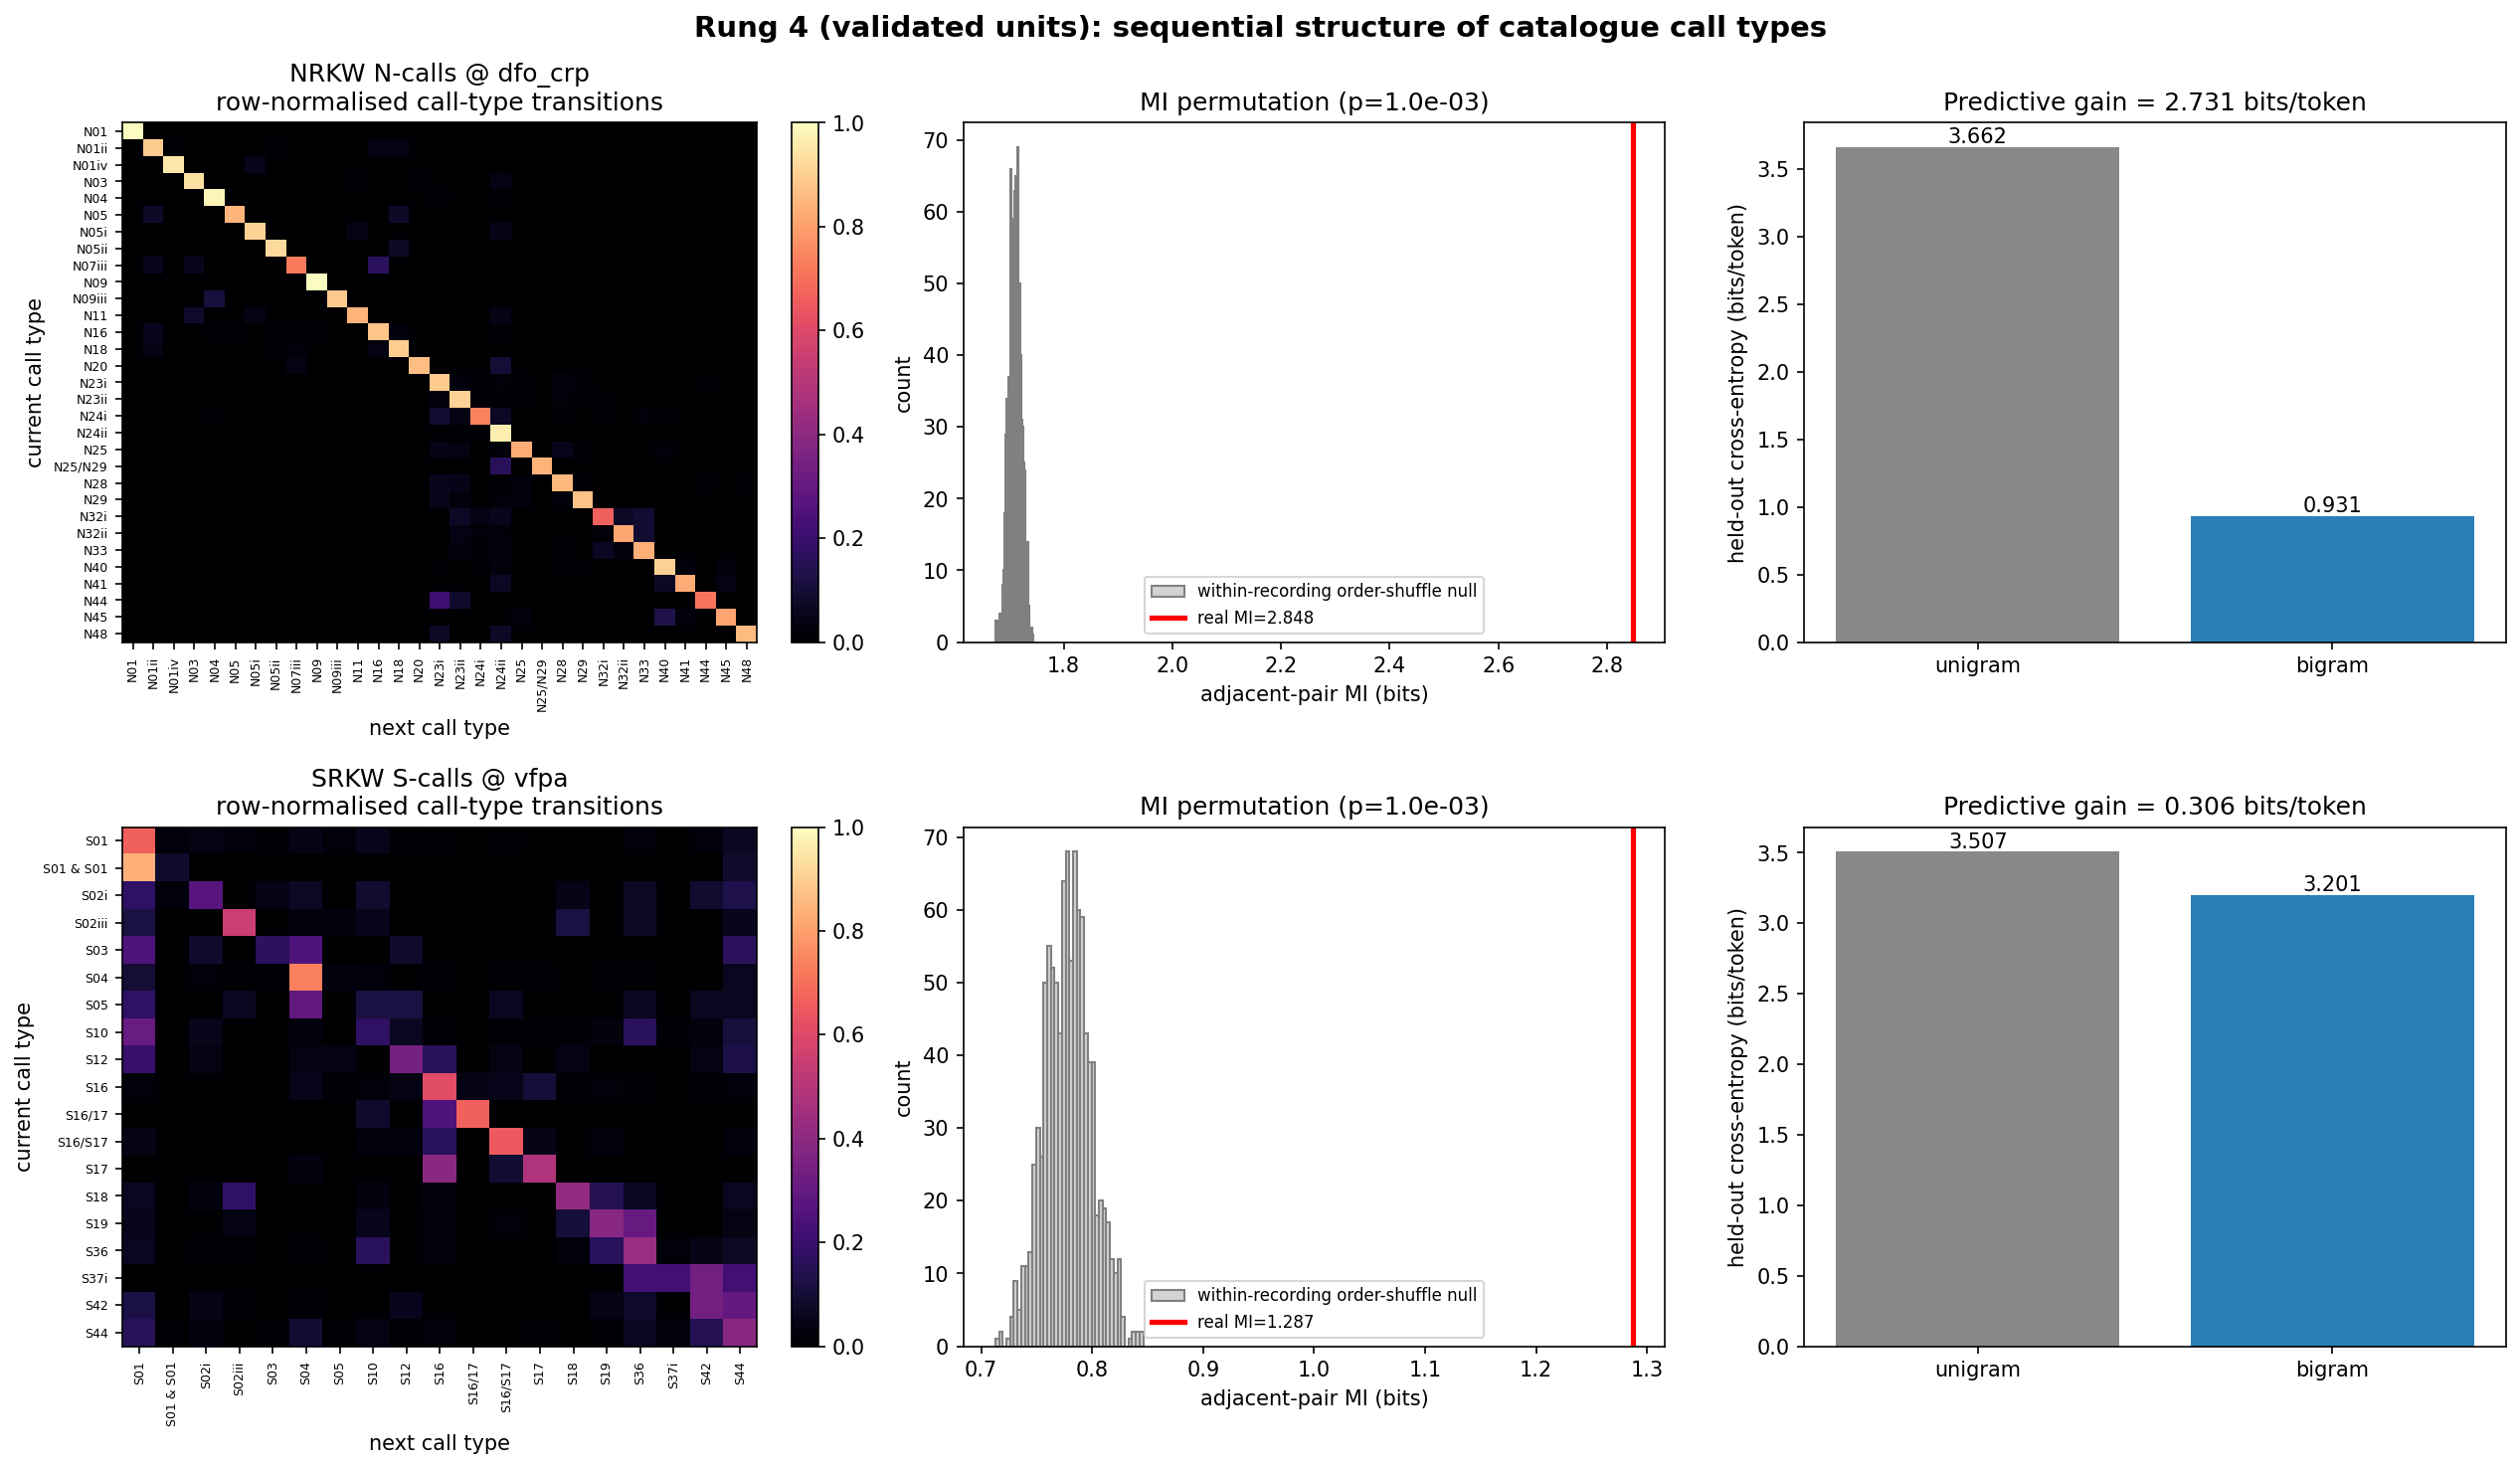
\includegraphics[width=\linewidth]{calltype_sequence.png}
\caption{Sequential structure over \emph{validated} catalogue call types, recording site held
constant. Top: Northern-Resident N-calls (DFO\_CRP, 31 types) -- row-normalised transition
matrix (left), adjacent-pair MI $2.85$ bits versus a within-recording order-shuffle null of
$1.71$ bits, $p=10^{-3}$ (middle), and a held-out bigram beating a unigram by $2.73$ bits/token
(right). Bottom: Southern-Resident S-calls (VFPA, 19 types), MI $1.29$ vs $0.78$ bits.}
\label{fig:calltypeseq}
\end{figure}

\begin{figure}[t]
\centering
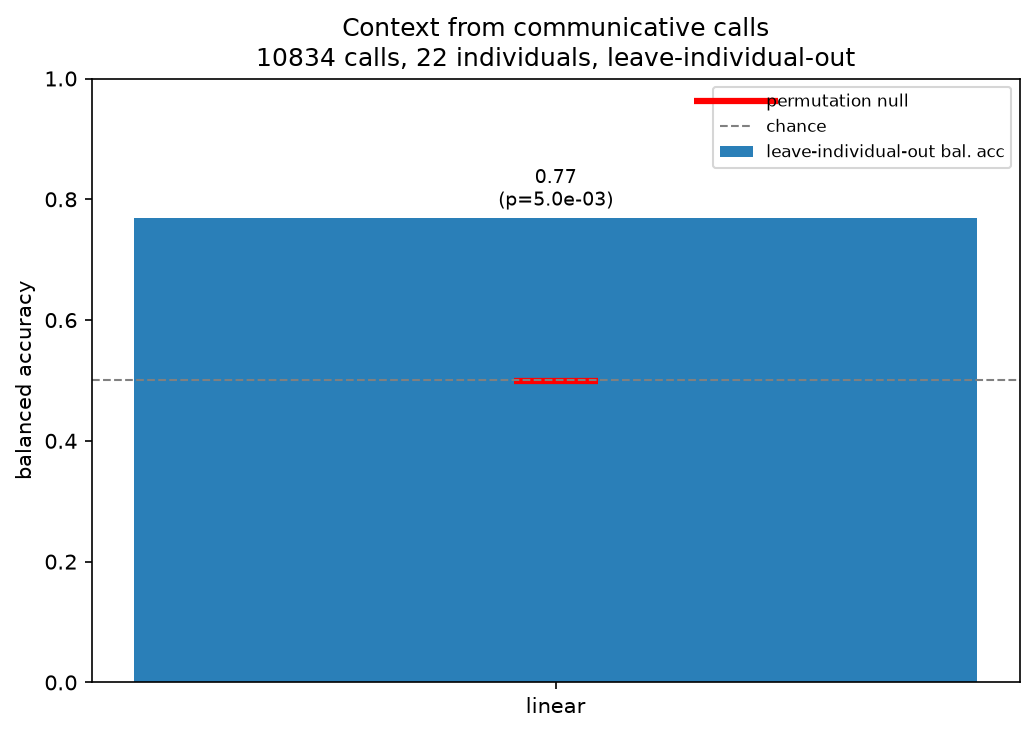
\includegraphics[width=\linewidth]{context_decode.png}
\caption{H5 (DTAG): communicative calls predict the caller's movement-defined behavioural
context (foraging vs.\ non-foraging) at $0.770$ balanced accuracy under leave-individual-out
cross-validation across 22 tagged whales ($10{,}834$ calls), against a label-permutation null
of $0.499 \pm 0.007$ ($p=5\times10^{-3}$). The context label uses tag depth and acceleration
only, so it is independent of the decoded call audio.}
\label{fig:context}
\end{figure}

\begin{figure}[t]
\centering
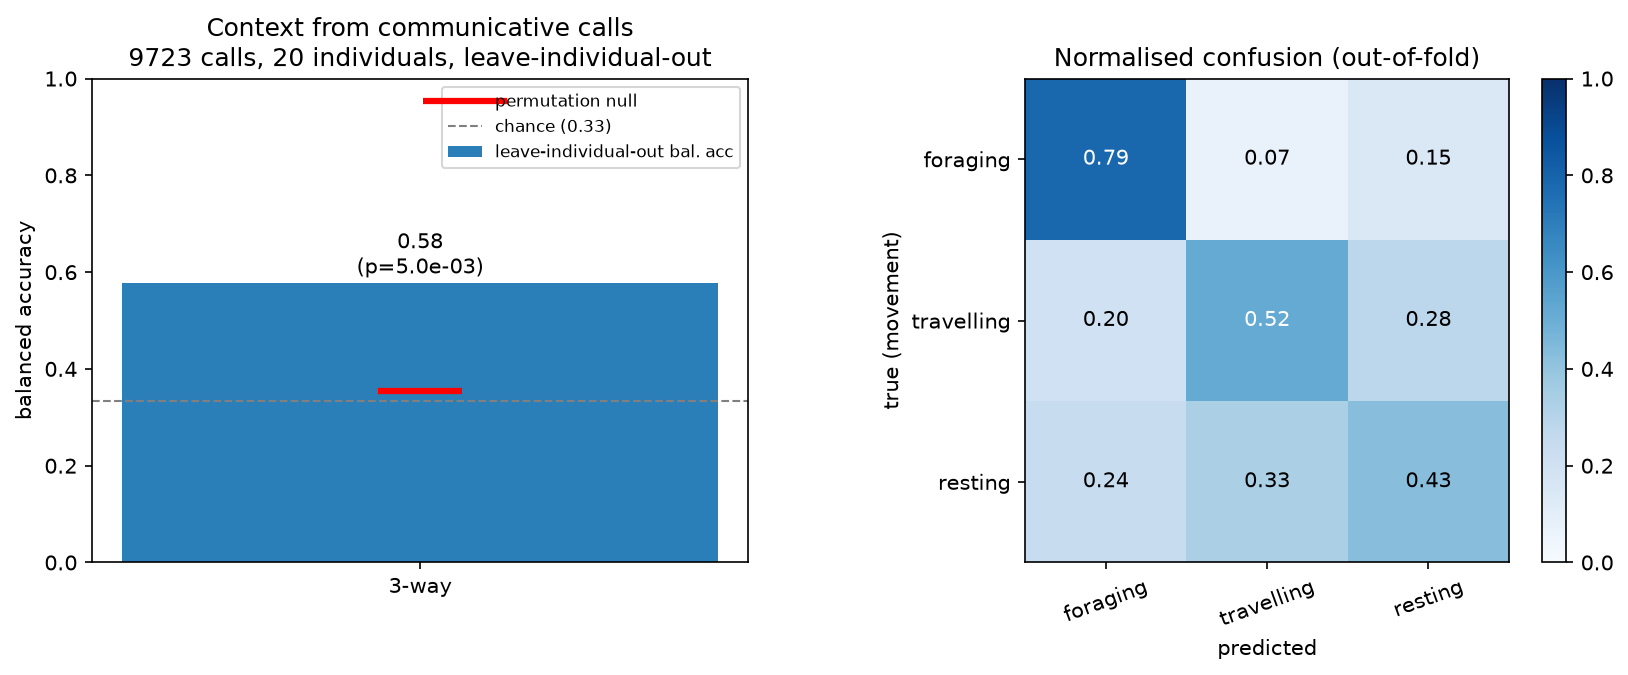
\includegraphics[width=\linewidth]{context3_decode.png}
\caption{H5 multi-context: a three-way foraging/travelling/resting decode (movement-only
labels; travelling/resting split by per-individual ODBA) reaches $0.577$ balanced accuracy
across the 20 whales carrying all three contexts (chance $0.333$; within-individual null
$0.355 \pm 0.008$, $p=5\times10^{-3}$). Right: out-of-fold confusion matrix; foraging is the
most separable context.}
\label{fig:context3}
\end{figure}

\begin{figure}[t]
\centering
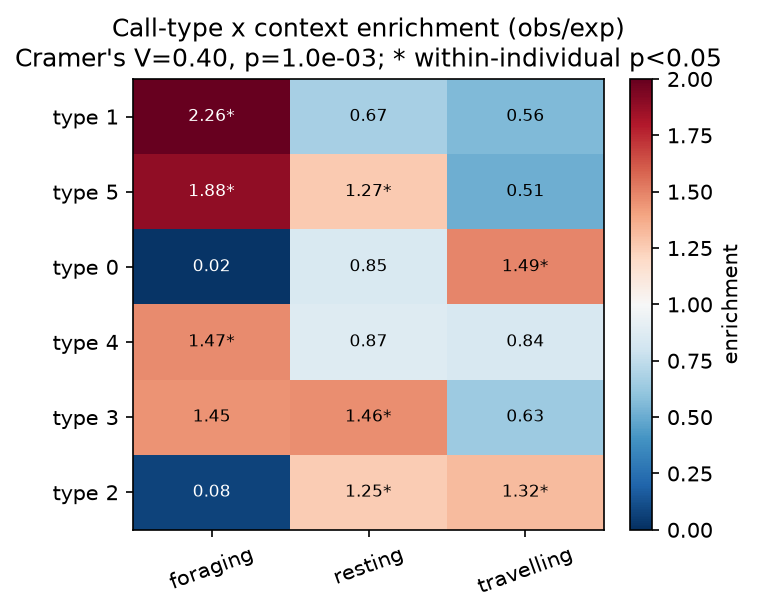
\includegraphics[width=0.92\linewidth]{calltype_context.png}
\caption{Call-type $\times$ context selectivity: data-driven call-type clusters are
over-represented in specific contexts (enrichment $=$ observed/expected; ${}^{*}$ within-individual
permutation $p<0.05$). Overall Cram\'er's $V=0.40$ against a within-individual shuffle null of
$0.08$ ($p<10^{-3}$) -- the production-side signature of context-specific calling.}
\label{fig:calltypectx}
\end{figure}

\begin{figure}[t]
\centering
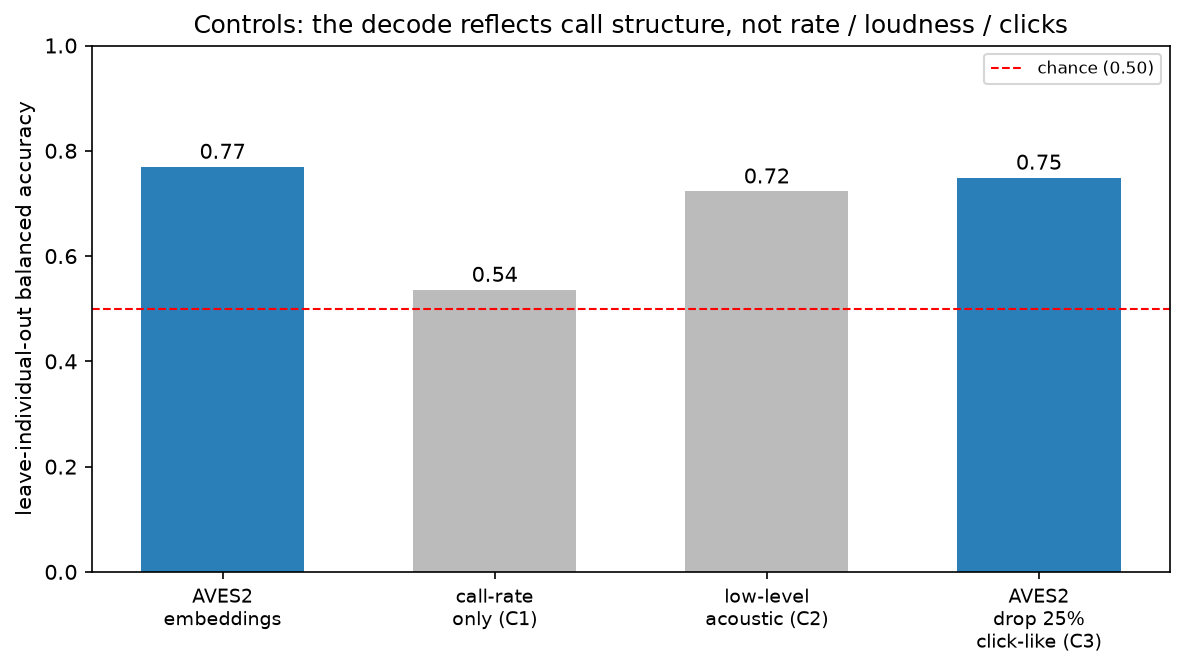
\includegraphics[width=0.85\linewidth]{context_controls.png}
\caption{H5 controls (binary contrast): the AVES2 call-embedding decode ($0.770$) is not
explained by call rate ($0.536$) or loudness ($0.577$), and survives discarding the $25\%$
most click-like clips ($0.749$); the signal is in call structure, not biosonar or calling
intensity.}
\label{fig:contextctrl}
\end{figure}

\begin{figure}[t]
\centering
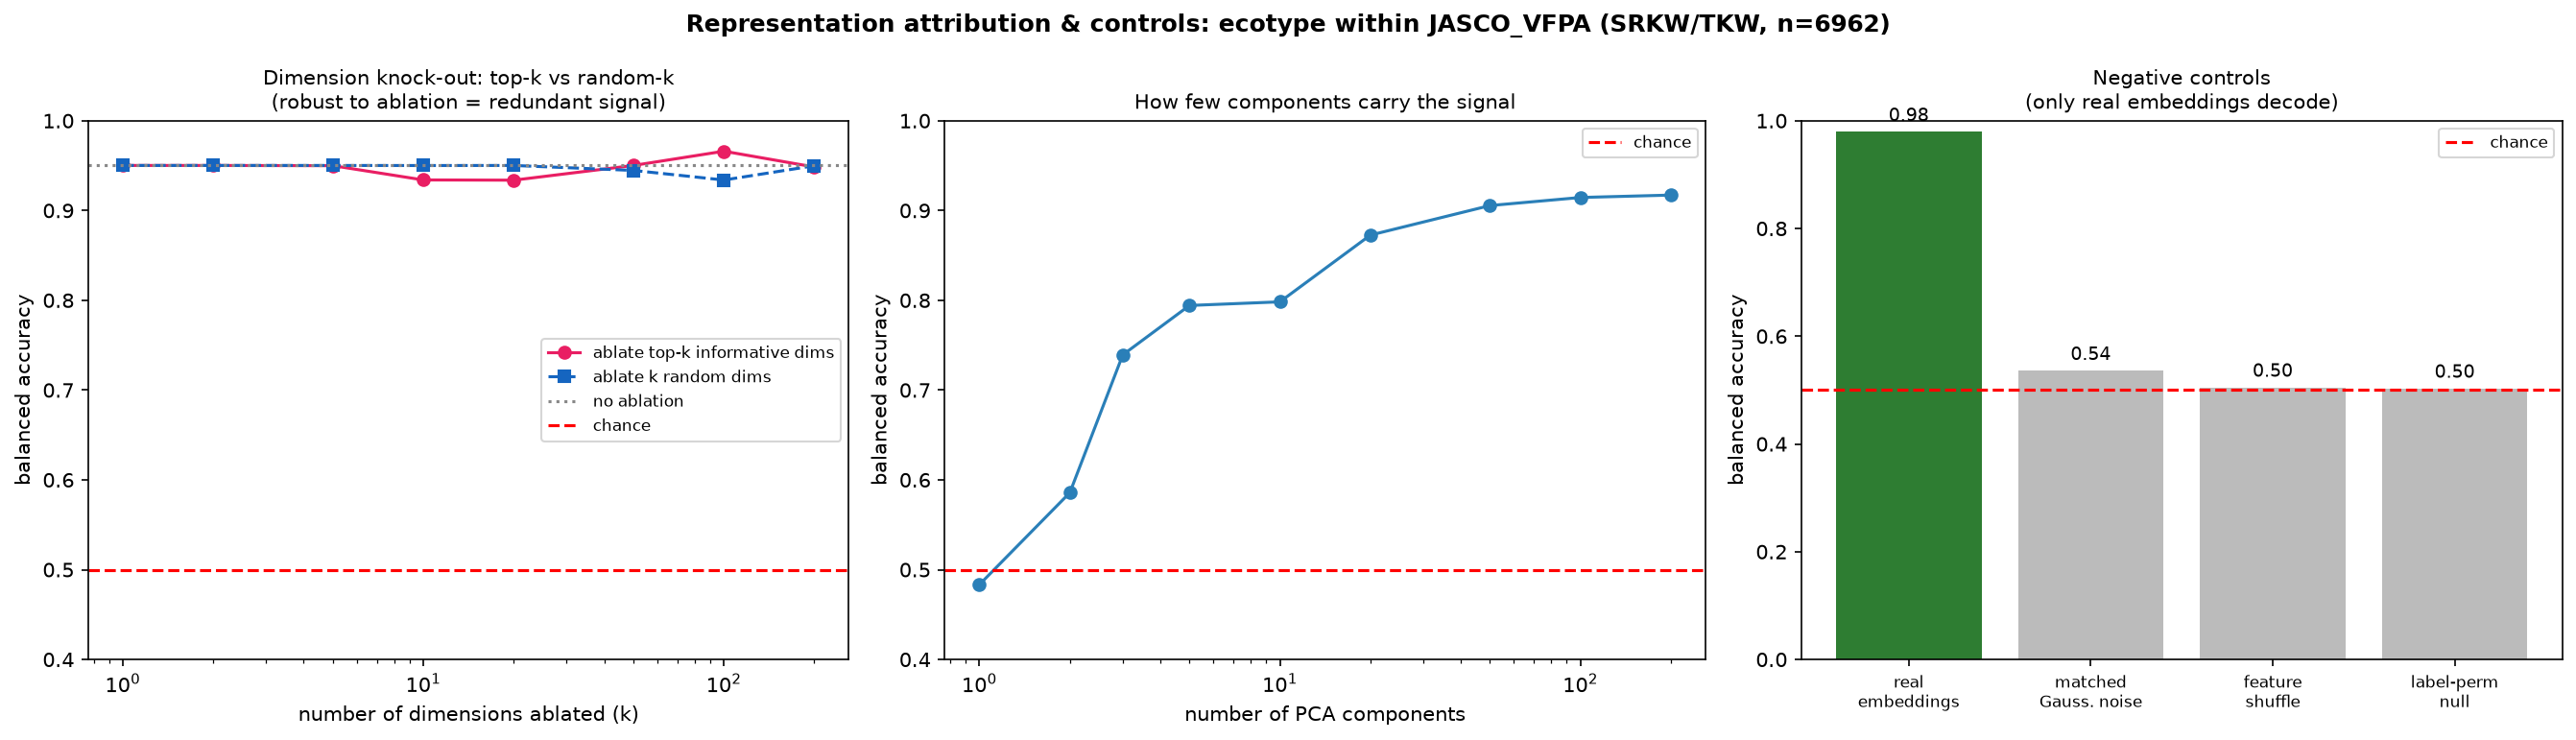
\includegraphics[width=\linewidth]{attribution_controls.png}
\caption{Representation attribution and negative controls for the within-site
SRKW/TKW decode. Left: ablating the top-$k$ permutation-important AVES2 dimensions does
not collapse the decode (it tracks random-$k$ ablation), so the signal is redundantly
distributed. Middle: a low-rank PCA projection already recovers most of the signal.
Right: structure-matched noise ($0.54$), feature shuffle ($0.51$), and the
label-permutation null ($0.50$) all sit near chance, far below the real embeddings
($0.98$).}
\label{fig:attribution}
\end{figure}

\section{Limitations}
The pooled $0.97$ figure is not a biological result and we do not report it as one; the
honest estimate is the within-site number. Cross-site transfer for ecotype is bounded by the
single-provider ecotype (SAR) and by absolute embedding-space shifts between sites. The
supervised call-type result covers the two resident populations (SRKW and NRKW) but not Bigg's
or offshore types; the catalogue labels are detection-level and correlate with pod and
matriline, so it is call-type discrimination, not evidence of meaning, and the cross-site
transfer estimate rests on a modest SMRU test set ($267$ calls, five shared types). Unsupervised structure is weak and reduction-dependent. The $k$-means sequence test is
complemented by the validated-call-type test (which uses expert catalogue labels and site
control), but both characterise call \emph{ordering}, not meaning, and the bouting-heavy
N-call streams show that much of the raw transition signal is repetition. The earlier
recording-level ``response-proxy'' and timing analyses retained in the repository are
exploratory associations, not segment-level behaviour and not responses to broadcast signals
\citep{wellard2020,wellard2020_appendix2}; they remain excluded from every claim here. The
behavioural-context decode (H5) is, by contrast, segment-level and individual-held-out, but
carries its own boundaries: the context labels are movement-only proxies, so foraging is a
dive-depth/prey-capture signature and the travelling/resting split is an ODBA activity
dichotomy rather than a named ethogram state (socialising or alarm are not resolved), and the
result is therefore an association between communicative-call structure and concurrent
behavioural context, not evidence of referential meaning. The call-type clusters are
data-driven partitions of the on-animal tag domain, not the named DCLDE catalogue types, and
the cluster structure is soft (low silhouette); the call-type-by-context association is robust
to this because its null reuses the same clustering. Echolocation is addressed by the
$16$\,kHz analysis band (which excludes click peak energy) and by the click-likeness control,
but on-tag attribution of calls to the focal whale is imperfect; and absolute call times
assume contiguous tag audio from the start of the movement record. Most fundamentally, this
remains an archival decoding study: it is non-invasive and uses the animals' endogenous
signals, and while H5 shows that communicative calls are produced context-specifically across
more than one behavioural context, it demonstrates neither referential call-level meaning nor
any measured response to a broadcast signal.

\paragraph{Arousal versus content.} A behavioural-context decode could in principle
reflect a graded arousal or activity axis rather than context-specific signal content. Two
features of the result argue against a pure-arousal account: the link is carried by
\emph{which} call types occur (call-type $\times$ context Cram\'er's $V=0.40$, specific
types enriched in specific contexts) rather than by a monotone intensity shift, and
loudness alone decodes context at only $0.577$ against the embeddings' $0.770$. We
nonetheless do not claim to have fully separated arousal from content, which would require
independent physiological or valence measures.

\paragraph{Calibrated confidence.} We attach graded confidence to each headline claim.
\emph{High}: frozen AVES2 embeddings encode within-site ecotype structure and
catalogue-validated call-type structure, and call-type identity transfers across
independent recording sites (multiple controls, both resident populations, structure
destroyed under matched-noise and feature-shuffle controls). \emph{Medium--high}:
communicative calls are produced context-specifically across more than one movement-defined
behavioural context with the individual held out (identity-controlled and multi-control,
but the labels are movement-only proxies and the on-tag call-type clusters are soft).
\emph{No claim (out of scope)}: referential call-level meaning, the perception side of
context-specificity, and any response to a broadcast signal.

\section{Reproducibility}
The repository provides exact commands, a hash-frozen artifact, per-head metrics JSON and
figures, a label audit, and a software snapshot. Each reported number is regenerated by the
\texttt{run\_h1\_probes.py}, \texttt{run\_h4\_confound.py}, \texttt{run\_h2\_clustering.py},
\texttt{run\_h3\_sequence\_lm.py}, \texttt{run\_sequence\_structure.py},
\texttt{run\_calltype\_discovery.py} and \texttt{run\_calltype\_model.py} scripts on the frozen
artifact, with the call-type manifest built by \texttt{build\_calltype\_manifest.py}; the
full-catalogue call-type encode and models are reproduced by
\texttt{notebooks/calltype\_encode\_colab.ipynb} (\texttt{reports/calltype\_model\_full\_summary.json}),
the validated-call-type sequence test by \texttt{run\_calltype\_sequence.py}
(\texttt{reports/calltype\_sequence\_summary.json}), and the public-data ceiling audit by
\texttt{fetch\_orcasound\_labels.py}. The behavioural-context decode (H5) is reproduced end to
end from public DTAG deposits by \texttt{dtag\_local\_extract.py} (downloads each tag archive,
losslessly decodes it, detects communicative calls, and cuts clips),
\texttt{dtag\_context\_labels.py} (builds the movement-only foraging/non-foraging label and
reports per-individual yield in \texttt{reports/context\_label\_yield.json}), and
\texttt{dtag\_context\_decode.py} (frozen-AVES2 encode, leave-individual-out decode,
permutation null; \texttt{reports/context\_decode\_summary.json},
\texttt{figures/context\_decode.png}). The multi-context strengthening is reproduced by
\texttt{dtag\_context\_multilabel.py} (three-state foraging/travelling/resting labels from
depth, jerk, and ODBA), \texttt{dtag\_context\_multidecode.py} (three-way leave-individual-out
decode and within-individual null; \texttt{reports/context3\_decode\_summary.json}),
\texttt{dtag\_calltype\_context.py} (call-type-by-context selectivity;
\texttt{reports/calltype\_context\_selectivity.json}), and \texttt{dtag\_context\_controls.py}
(rate/loudness/low-level/echolocation controls; \texttt{reports/context\_controls\_summary.json}),
all reusing the frozen-AVES2 call embeddings so no re-encoding is required. The
representation attribution and negative-control battery are reproduced by
\texttt{run\_attribution\_controls.py} (\texttt{reports/attribution\_controls\_summary.json},
\texttt{figures/attribution\_controls.png}). Raw audio and tag
archives are downloaded from public
sources and excluded from version control.

\section{Future work}
A site-controlled decoding baseline is the credible foundation for the next scientific step:
pairing these embeddings with field groups capable of in-situ playbacks to test whether
specific call structures elicit measurable, context-specific responses, as demonstrated for
dolphins \citep{sayigh2025nsw}. We release the pipeline to make that collaboration
concrete and reproducible.

\bibliographystyle{plainnat}
\bibliography{refs}

\end{document}
